\documentclass[11pt,a4paper]{article}
\usepackage[T1]{fontenc}
\usepackage[utf8]{inputenc}
\usepackage[french]{babel}
\usepackage{geometry}
\geometry{margin=2.5cm}
\usepackage{xcolor}
\usepackage{booktabs}
\usepackage{array}
\usepackage{graphicx}
\usepackage{tikz}
\usetikzlibrary{shapes.geometric,arrows.meta,positioning,fit}
\usepackage{fancyhdr}
\usepackage{hyperref}
\usepackage{listings}
\usepackage{amsmath}
\usepackage{longtable}

\hypersetup{colorlinks=true,linkcolor=blue,urlcolor=blue,citecolor=blue}

\lstset{
  basicstyle=\ttfamily\small,
  breaklines=true,
  frame=single,
  backgroundcolor=\color{gray!8},
  columns=fullflexible,
}

\graphicspath{{figures_campaign2/}}
\setlength{\headheight}{14pt}
\pagestyle{fancy}
\fancyhf{}
\fancyhead[L]{Campagne 2 --- Percolation vs. stabilité thermodynamique}
\fancyhead[R]{\thepage}
\renewcommand{\headrulewidth}{0.4pt}

\title{\bfseries Poids de percolation et stabilité thermodynamique \\
sur un jeu de 186 composés \\
\large Campagne 2 : construction du jeu de données, calcul VASP+LOBSTER,
et analyse statistique}
\author{Gilles Frapper \\ Professeur des Universités, Chimie Théorique \\ IC2MP UMR 7285 CNRS, Université de Poitiers \\ \href{mailto:gilles.frapper@univ-poitiers.fr}{gilles.frapper@univ-poitiers.fr}\\[4pt] \small Rapport généré dans le cadre du projet \texttt{viability}}
\date{14 août 2026}

\begin{document}
\maketitle

\tableofcontents
\newpage

\section{Objectif et problématique}

Le premier rapport (6 composés jouets) avait établi que le descripteur de
percolation calculé par \texttt{percolation\_path.py} diverge fortement des
agrégats ICOHP classiques (somme, moyenne, min, max), sans toutefois
disposer d'un échantillon assez grand pour tester statistiquement si cette
différence est \emph{utile} : le descripteur de percolation apporte-t-il une
information prédictive sur la stabilité thermodynamique
(\texttt{energy\_above\_hull}) que les agrégats classiques n'apportent pas
déjà ?

Cette deuxième campagne construit un jeu de données de 186 composés
(180 nouveaux + les 6 composés pilotes) réparti en trois familles :
\begin{itemize}
  \item \textbf{exp\_stable} : composés expérimentaux (référencés ICSD) sur
    le hull convexe thermodynamique de Materials Project ;
  \item \textbf{exp\_metastable} : composés expérimentaux métastables
    ($0 < E_\text{hull} \leq 100$~meV/atome) ;
  \item \textbf{theo\_metastable} : composés théoriques (jamais observés
    expérimentalement) métastables ($0 < E_\text{hull} \leq 200$~meV/atome).
\end{itemize}

La distinction \texttt{exp\_metastable} / \texttt{theo\_metastable} sert de
proxy pour la persistance cinétique : un composé métastable observé
expérimentalement a, par définition, survécu assez longtemps pour être
synthétisé et caractérisé, contrairement à un composé théorique de même
métastabilité thermodynamique.

\section{Méthodologie}

\subsection{Sélection du jeu de données}

Requête Materials Project (\texttt{mp\_dataset/select\_campaign.py}) :
systèmes chimiques unaires et binaires, non magnétiques
($|\text{aimantation totale}| \leq 0.01~\mu_B$/unité formulaire --- le champ
catégoriel \texttt{magnetic\_ordering} de MP est \og{}Unknown\fg{} pour
$\sim$98\% des entrées et aurait exclu la quasi-totalité des composés
réellement non magnétiques), sans éléments f, $\leq 20$ atomes/maille,
60 composés par famille avec un plafond de 2 entrées par système chimique
(\texttt{chemsys}) pour garantir une diversité élémentaire plutôt qu'une
accumulation de polymorphes d'un même système.

\subsection{Classification du type de liaison}

Le type de liaison (ionique / covalent / métallique) est calculé par la
fonction \texttt{classify()} de \texttt{fetch\_candidates.py}
(\textbf{réutilisée sans modification}, conformément à la consigne de la
campagne), à partir de \texttt{is\_metal} et de la composition élémentaire.
Cette classification est un axe secondaire d'analyse ici, pas l'axe
d'échantillonnage principal (contrairement à la proposition initiale de
plan de campagne, remplacée à la demande de l'utilisateur par le schéma
stable/métastable ci-dessus).

\subsection{Calcul VASP + LOBSTER}

Même gabarit que la campagne pilote (calcul statique, \texttt{ISYM=$-1$},
\texttt{LASPH=.TRUE.}, potentiels PAW-PBE recommandés par
\texttt{pymatgen.io.vasp.sets.MPRelaxSet}), avec deux améliorations :
\texttt{NBANDS} n'est plus une valeur fixe mais dérivée par composé du
nombre d'orbitales locales de la base LOBSTER
(\texttt{Lobsterin.write\_INCAR}), et la détermination des fonctions de
base passe par \texttt{Lobsterin.get\_basis(potcar\_symbols=\ldots)}
plutôt que par le parsing direct du fichier POTCAR (dont la validation
interne de \texttt{pymatgen} échoue sur plusieurs POTCAR non reconnus par
empreinte de hachage dans le miroir local).

\subsection{Statistiques}

Corrélation de Spearman (pas de raison d'attendre une relation linéaire)
entre le poids de percolation (brut et normalisé par
$|\text{ICOHP}_\text{min}|$) et \texttt{energy\_above\_hull}, globalement et
par type de liaison ; même chose pour les agrégats ICOHP classiques, pour
comparaison directe ; régression logistique de référence (stable vs.
métastable, 2--3 variables, validation croisée 5 plis) pour une AUC de
référence. \textbf{Aucun SISSO, aucune régression symbolique} : prématuré
avec un seul descripteur candidat et cet ordre de grandeur d'échantillon
(voir \S\ref{sec:limites}).

\section{Organigramme du workflow}

\begin{center}
\begin{tikzpicture}[
  node distance=0.75cm and 1.6cm,
  box/.style={draw, rounded corners, minimum width=5.0cm, minimum height=1.0cm,
              align=center, fill=blue!6, font=\small},
  io/.style={draw, minimum width=5.0cm, minimum height=1.0cm, align=center,
             fill=orange!10, font=\small},
  arr/.style={-{Latex[length=2.2mm]}, thick}
]
\node[io]  (mp)     {Materials Project (API) \\ 180 composés (3 familles $\times$ 60)};
\node[box, below=of mp] (prep)   {\texttt{download\_campaign.py} + \texttt{prepare\_vasp\_lobster.py} \\ POSCAR, INCAR, KPOINTS, POTCAR, lobsterin};
\node[box, below=of prep] (slurm)  {SLURM (\texttt{submit\_array.sh}) \\ tableau plafonné à 8 t\^aches concurrentes};
\node[box, below=of slurm] (vasplob) {VASP (statique) $\rightarrow$ LOBSTER 5.1.1 \\ ICOHPLIST.lobster, ICOBILIST.lobster};
\node[box, below=of vasplob] (perc)   {\texttt{percolation\_path.py} (inchang\'e) \\ 186 composés (180 + 6 pilotes)};
\node[box, below=of perc] (join)   {\texttt{analysis/build\_dataset.py} \\ jointure + descripteur normalisé + bond\_type};
\node[io, below=of join] (stats)  {\texttt{analysis/stats\_analysis.py} \\ corrélations, régression logistique, figures};

\draw[arr] (mp) -- (prep);
\draw[arr] (prep) -- (slurm);
\draw[arr] (slurm) -- (vasplob);
\draw[arr] (vasplob) -- (perc);
\draw[arr] (perc) -- (join);
\draw[arr] (join) -- (stats);
\end{tikzpicture}
\end{center}

\section{Environnement}

Identique à la campagne pilote (Yargla, VASP 6.5.0, LOBSTER 5.1.1,
\texttt{.venv} Python 3.11), complété par :
\texttt{mp-api}, \texttt{pandas}, \texttt{scipy}, \texttt{scikit-learn},
\texttt{matplotlib} (voir \texttt{requirements.txt}).

\section{Jeu de données}

\begin{center}
\begin{tabular}{@{}lrl@{}}
\toprule
Famille & $n$ & Plage $E_\text{hull}$ (eV/atome) \\
\midrule
exp\_stable      & 63 & 0.0000 (par construction) \\
exp\_metastable  & 63 & 0.0005 -- 0.0907 \\
theo\_metastable & 60 & 0.0013 -- 0.1991 \\
\bottomrule
\end{tabular}

\vspace{0.3cm}

\begin{tabular}{@{}lr@{}}
\toprule
Type de liaison (\texttt{classify()}) & $n$ \\
\midrule
métallique       & 88 \\
covalent         & 23 \\
ionique          & 9 \\
non classifié    & 66 \\
\bottomrule
\end{tabular}
\end{center}

35\% des composés (66/186) ne correspondent à aucune des trois catégories
de \texttt{classify()} --- principalement des pnictures/chalcogénures de
métaux de transition et des composés hydrogénés, une limite réelle de
l'heuristique réutilisée telle quelle, documentée mais non corrigée ici.

\section{Résultats}

\subsection{Corrélations (Spearman)}

\begin{center}
\small
\begin{tabular}{@{}llrrr@{}}
\toprule
Groupe & Métrique & $n$ & $\rho$ & $p$ \\
\midrule
tous & poids percolation (brut)       & 186 & 0.064 & 0.383 \\
tous & poids percolation (normalisé)  & 186 & 0.071 & 0.339 \\
métallique & poids percolation (brut)      & 88 & 0.191 & 0.075 \\
métallique & poids percolation (normalisé) & 88 & \textbf{0.222} & \textbf{0.038} \\
ionique$^*$ & poids percolation (brut)     & 9  & $-$0.402 & 0.284 \\
covalent & poids percolation (brut)        & 23 & 0.165 & 0.453 \\
\midrule
tous & ICOHP somme    & 186 & 0.032 & 0.670 \\
tous & ICOHP min      & 186 & 0.093 & 0.209 \\
métallique & ICOHP somme  & 88 & 0.223 & 0.037 \\
métallique & ICOHP min    & 88 & 0.198 & 0.065 \\
\bottomrule
\end{tabular}

\footnotesize $^*$ $n<15$ : à ne pas surinterpréter.
\end{center}

Dans le seul sous-groupe où un résultat atteint la significativité nominale
(métallique, $n=88$), le poids de percolation normalisé ($\rho=0.222$,
$p=0.038$) et la somme des ICOHP ($\rho=0.223$, $p=0.037$) sont
statistiquement indiscernables en force. \textbf{Le descripteur de
percolation n'apporte pas d'avantage prédictif démontré par rapport aux
agrégats classiques sur ce jeu de données} --- une réponse plus précise
que la formulation \og{}qualitativement différent\fg{} du rapport
précédent (6 composés), et plus directement exploitable.

\subsection{Régression logistique de référence}

Stable (hull) vs. métastable, variables : poids de percolation normalisé,
ICOHP moyen, indicatrices de type de liaison ($n=120$ après exclusion des
composés non classifiés).

\begin{center}
\begin{tabular}{@{}lr@{}}
\toprule
AUC (validation croisée, 5 plis) & $0.496 \pm 0.141$ \\
AUC par pli & 0.556, 0.430, 0.252, 0.637, 0.607 \\
\bottomrule
\end{tabular}
\end{center}

AUC $\approx 0.5$ : niveau du hasard. La dispersion importante entre plis
(0.25--0.64) indique elle-même l'absence de signal stable et apprenant à
cette taille d'échantillon, pas seulement un signal \og{}faible mais
réel\fg{}.

\subsection{Figures}

\begin{center}
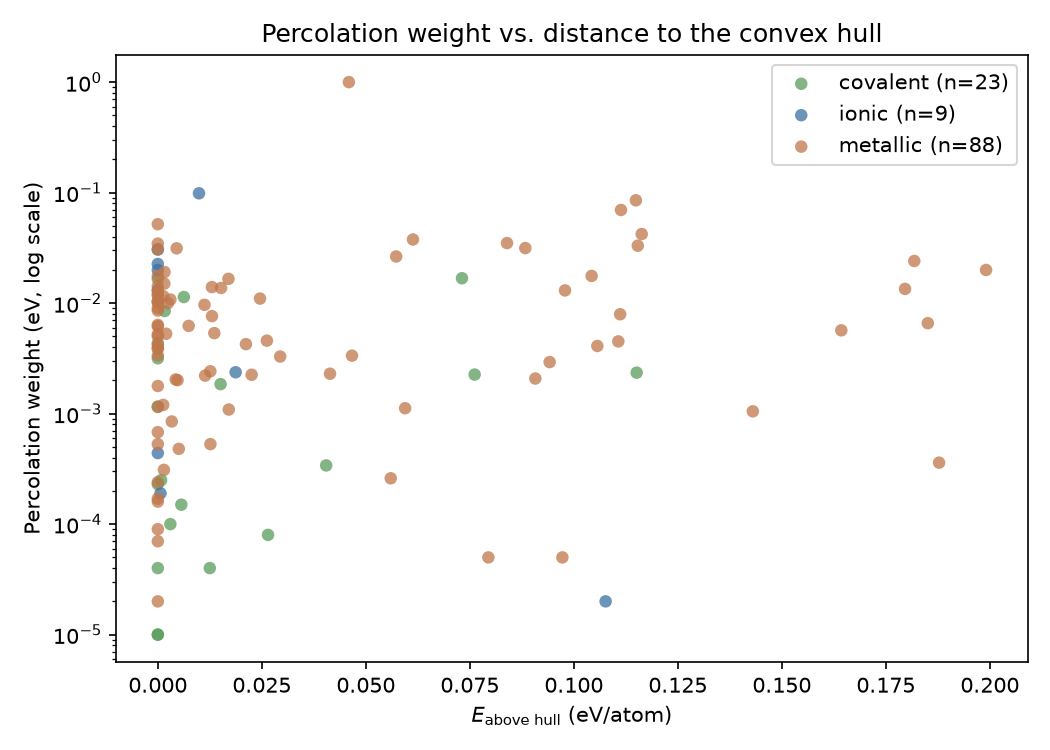
\includegraphics[width=0.85\textwidth]{percolation_vs_ehull.png}
\end{center}

\begin{center}

\includegraphics[width=0.55\textwidth]{roc_stable_vs_metastable.png}
\end{center}

\section{Incidents résolus}

Conformément à la consigne (\og{}chaque échec de job doit être loggé avec la
raison probable\fg{}), 5 des 178 jobs soumis en tableau SLURM ont échoué au
premier passage, tous diagnostiqués et corrigés à la source :

\begin{itemize}
  \item \textbf{Al12W, BW, WO2, TcW, TiW} (tous contenant du tungstène) :
    le POTCAR \texttt{W\_sv} du miroir local est dépourvu de son champ
    \texttt{LEXCH} (confirmé par inspection directe --- présent pour toutes
    les autres variantes testées, y compris \texttt{W} simple), ce que VASP
    interprète comme une fonctionnelle d'échange-corrélation incompatible
    et refuse d'exécuter. Corrigé en remplaçant la substitution
    \texttt{W\_sv} par \texttt{W} (PBE valide, vérifié).
  \item \textbf{Al12W} a échoué une seconde fois après cette correction,
    avec un SIGSEGV VASP --- exactement le problème connu signalé dans la
    mission (\texttt{ulimit -s unlimited} avant \texttt{vasp\_std}), présent
    dans \texttt{submit\_array.sh} mais oublié dans le gabarit SLURM
    individuel de \texttt{prepare\_vasp\_lobster.py}. Corrigé ; récupéré au
    second essai.
\end{itemize}

Taux de succès final : \textbf{186/186}.

\section{Coût de calcul}

\begin{center}
\begin{tabular}{@{}lrr@{}}
\toprule
 & VASP & LOBSTER \\
\midrule
Moyenne (s) & 124 & 397 \\
Médiane (s) & 72 & 145 \\
Maximum (s) & 1440 & 6675 \\
Total séquentiel & 6.4 h & 19.1 h \\
\bottomrule
\end{tabular}
\end{center}

Temps réel écoulé (parallélisme 8 tâches) : $\sim$3.5~h, dans le budget de
6~h fixé pour la nuit.

\section{Limites et perspectives}
\label{sec:limites}

\begin{itemize}
  \item \textbf{Taille d'échantillon} : 186 au total, mais 88/23/9 par type
    de liaison une fois stratifié --- les corrélations \og{}ioniques\fg{}
    ($n=9$) ne sont pas interprétables.
  \item \textbf{Maille primitive vs. conventionnelle} (héritée du rapport
    pilote) : non retraitée ici. C'est probablement la cause la plus
    probable de la faiblesse des corrélations observées --- la liaison la
    plus forte peut être entièrement intra-maille et ne contribuer à aucun
    cycle non contractile, biaisant le \og{}maillon faible\fg{} mesuré.
  \item \textbf{Pas de classe \og{}instable\fg{} au sens dynamique} :
    \texttt{theo\_metastable} est un proxy (composé jamais synthétisé), pas
    un résultat de calcul de phonons.
  \item \textbf{Couverture de \texttt{classify()}} : 35\% des composés non
    classifiés.
  \item \textbf{Pourquoi pas SISSO maintenant} : un seul descripteur
    candidat (le poids de percolation, sous deux variantes algébriquement
    liées), comparé à des agrégats eux-mêmes fonctions des mêmes valeurs
    ICOHP sous-jacentes --- aucun espace combinatoire de recherche
    significatif à ce stade. Justifier SISSO demanderait : (a) plusieurs
    descripteurs candidats conceptuellement nouveaux, (b) un $n$ par strate
    d'au moins 50--100, (c) un signal plus net qu'une AUC $\approx 0.5$.
\end{itemize}

\section{Conclusion}

Le jeu de données de 186 composés a été construit, calculé (VASP+LOBSTER)
et analysé de bout en bout, avec deux incidents de calcul diagnostiqués et
corrigés à la source. Le résultat principal est un résultat \emph{négatif}
mais chiffré et honnête : à cette taille d'échantillon, le descripteur de
percolation ne montre pas de corrélation significative avec la stabilité
thermodynamique, et n'apporte pas d'avantage démontré sur les agrégats
ICOHP classiques. Les actions prioritaires (\S\ref{sec:limites}) --- en
particulier le retraitement en maille conventionnelle et l'extension ciblée
du sous-échantillon métallique --- sont susceptibles de faire évoluer ce
résultat avant d'envisager un outillage de type SISSO.

\vspace{1cm}
\noindent\textit{Code source :} \url{https://github.com/John-Akapulco/viability} \\
\noindent\textit{Données :} \texttt{analysis/percolation\_vs\_hull.csv} \\
\noindent\textit{Rapport détaillé :} \texttt{analysis/REPORT.md}

\appendix
\section{Liste des composés}

Les 186 composés du jeu de données, classés par catégorie (famille), avec
leur identifiant Materials Project, leur distance au hull thermodynamique
(PBE, \texttt{energy\_above\_hull}) et le poids de percolation ICOHP
minimal (\texttt{icohp\_percolation\_weight\_min}, la métrique principale
de ce travail). Généré automatiquement depuis
\texttt{analysis/percolation\_vs\_hull.csv} par
\texttt{report/gen\_appendix.py}.

{\small
\begin{longtable}{@{}l l l r r@{}}
\caption{Liste compl\`ete des 186 compos\'es, class\'es par cat\'egorie, avec identifiant Materials Project, distance au hull (PBE), et poids de percolation ICOHP minimal.}\label{tab:appendix-compounds}\\
\toprule
Formule & mp-id & Liaison & $E_\text{hull}$ (eV/at) & Poids percolation (eV) \\
\midrule
\endfirsthead
\multicolumn{5}{@{}l}{\tablename\ \thetable\ (suite)}\\
\toprule
Formule & mp-id & Liaison & $E_\text{hull}$ (eV/at) & Poids percolation (eV) \\
\midrule
\endhead
\bottomrule
\endfoot
\multicolumn{5}{@{}l}{\textbf{Exp\'erimental, stable (hull)} ($n=63$)} \\
\midrule
As2S3 & mp-1189572 & covalent & 0.0000 & 1.00e-05 \\
AsF3 & mp-28027 & covalent & 0.0000 & 0.00e+00 \\
BI3 & mp-23189 & covalent & 0.0000 & 1.00e-05 \\
BW & mp-7832 & -- & 0.0000 & 1.90e-04 \\
BaAu2 & mp-30363 & m\'etallique & 0.0000 & 5.19e-02 \\
BaCl2 & mp-568662 & ionique & 0.0000 & 1.31e-02 \\
BaH2 & mp-23715 & -- & 0.0000 & 2.40e-04 \\
Be2Cu & mp-2031 & m\'etallique & 0.0000 & 1.15e-03 \\
Be2Nb3 & mp-11272 & m\'etallique & 0.0000 & 6.36e-03 \\
Be2V & mp-11281 & m\'etallique & 0.0000 & 6.80e-04 \\
CaAl4 & mp-1749 & m\'etallique & 0.0000 & 1.03e-02 \\
CaSn & mp-2450 & m\'etallique & 0.0000 & 5.23e-03 \\
CdPd & mp-1696 & m\'etallique & 0.0000 & 9.00e-05 \\
CoB & mp-20857 & -- & 0.0000 & 6.00e-05 \\
Cs2As3 & mp-15557 & -- & 0.0000 & 2.02e-02 \\
FeS & mp-505531 & -- & 0.0000 & 3.05e-03 \\
Ge2Os & mp-10032 & m\'etallique & 0.0000 & 1.21e-02 \\
HfTc2 & mp-1095669 & m\'etallique & 0.0000 & 1.77e-02 \\
Hg4Pt & mp-936 & m\'etallique & 0.0000 & 3.36e-03 \\
HgF2 & mp-8177 & -- & 0.0000 & 8.95e-03 \\
InBr & mp-22870 & covalent & 0.0000 & 1.02e-02 \\
KI & mp-22898 & ionique & 0.0000 & 2.26e-02 \\
KN3 & mp-827 & -- & 0.0000 & 2.80e-04 \\
Li2Se & mp-2286 & -- & 0.0000 & 1.16e-02 \\
LiB & mp-1001835 & -- & 0.0000 & 2.91e-03 \\
Mg2Ni & mp-2137 & m\'etallique & 0.0000 & 1.60e-04 \\
MgP4 & mp-384 & -- & 0.0000 & 0.00e+00 \\
MnAl12 & mp-1104165 & m\'etallique & 0.0000 & 1.42e-02 \\
MoSe2 & mp-1634 & covalent & 0.0000 & 1.16e-03 \\
NaS & mp-2400 & -- & 0.0000 & 0.00e+00 \\
Na & mp-10172 & -- & 0.0000 & 1.97e-03 \\
Nb3Ir & mp-1458 & m\'etallique & 0.0000 & 9.02e-03 \\
NbGa3 & mp-1973 & m\'etallique & 0.0000 & 8.58e-03 \\
PI2 & mp-29443 & covalent & 0.0000 & 2.30e-04 \\
PbSe & mp-2201 & covalent & 0.0000 & 1.66e-02 \\
RbI & mp-22903 & ionique & 0.0000 & 2.00e-02 \\
Sc5Ge3 & mp-17190 & m\'etallique & 0.0000 & 5.30e-04 \\
ScAg2 & mp-1018128 & m\'etallique & 0.0000 & 1.70e-04 \\
ScTe & mp-10026 & -- & 0.0000 & 7.12e-03 \\
SnPt & mp-19856 & m\'etallique & 0.0000 & 1.29e-02 \\
SrO2 & mp-2697 & ionique & 0.0000 & 4.40e-04 \\
SrSi & mp-2661 & m\'etallique & 0.0000 & 7.00e-05 \\
Ta5Ge3 & mp-17593 & m\'etallique & 0.0000 & 3.46e-02 \\
TaP & mp-1067587 & -- & 0.0000 & 3.14e-02 \\
TaSb2 & mp-11697 & m\'etallique & 0.0000 & 1.17e-02 \\
Te2Pd & mp-782 & -- & 0.0000 & 1.44e-02 \\
Te2Ru & mp-267 & covalent & 0.0000 & 4.34e-03 \\
TeO2 & mp-8377 & covalent & 0.0000 & 4.00e-05 \\
Ti3In & mp-866046 & m\'etallique & 0.0000 & 5.01e-03 \\
Ti3Pt & mp-2339 & m\'etallique & 0.0000 & 1.78e-03 \\
TiBe12 & mp-1104067 & m\'etallique & 0.0000 & 2.40e-04 \\
TiNi & mp-1048 & m\'etallique & 0.0000 & 3.91e-03 \\
TiO & mp-1071163 & -- & 0.0000 & 6.40e-04 \\
TiSi2 & mp-1077503 & m\'etallique & 0.0000 & 6.18e-03 \\
TlCl & mp-571079 & -- & 0.0000 & 7.17e-03 \\
VNi2 & mp-11531 & m\'etallique & 0.0000 & 3.88e-03 \\
WO2 & mp-1524394 & -- & 0.0000 & 2.20e-04 \\
Zr2Au & mp-2348 & m\'etallique & 0.0000 & 3.06e-02 \\
Zr5Pb3 & mp-681992 & m\'etallique & 0.0000 & 2.00e-05 \\
ZrMo2 & mp-2049 & m\'etallique & 0.0000 & 1.05e-02 \\
Si & mp-149 & covalent & 0.0000 & 3.17e-03 \\
NaCl & mp-22862 & ionique & 0.0000 & 3.07e-02 \\
AlNi & mp-1487 & m\'etallique & 0.0000 & 4.19e-03 \\
\midrule
\multicolumn{5}{@{}l}{\textbf{Exp\'erimental, m\'etastable} ($n=63$)} \\
\midrule
CdI2 & mp-567259 & -- & 0.0005 & 2.38e-02 \\
MgCl2 & mp-570259 & ionique & 0.0006 & 1.90e-04 \\
C & mp-169 & covalent & 0.0008 & 2.50e-04 \\
ZrBr & mp-1065846 & -- & 0.0008 & 7.88e-03 \\
Li3Hg & mp-1646 & m\'etallique & 0.0013 & 1.20e-03 \\
Ta7Co6 & mp-1104548 & m\'etallique & 0.0015 & 3.10e-04 \\
CaGa4 & mp-2461 & m\'etallique & 0.0016 & 1.91e-02 \\
InCl & mp-571636 & covalent & 0.0016 & 8.50e-03 \\
NiB & mp-14019 & -- & 0.0018 & 4.10e-04 \\
MgH2 & mp-23711 & -- & 0.0019 & 1.00e-05 \\
Sn7Ir5 & mp-20466 & m\'etallique & 0.0024 & 1.00e-02 \\
NaN3 & mp-1066400 & -- & 0.0029 & 7.00e-04 \\
ClF3 & mp-556767 & -- & 0.0030 & 0.00e+00 \\
SiS2 & mp-1095294 & covalent & 0.0030 & 1.00e-04 \\
Sr5Sn3 & mp-17720 & m\'etallique & 0.0030 & 1.08e-02 \\
Te2Ir & mp-1551 & -- & 0.0030 & 2.80e-03 \\
Li13Sn5 & mp-30769 & m\'etallique & 0.0033 & 8.50e-04 \\
H3N & mp-643432 & covalent & 0.0038 & 0.00e+00 \\
Cs2Se & mp-1011696 & -- & 0.0042 & 2.62e-02 \\
In3Ir & mp-630976 & m\'etallique & 0.0043 & 2.04e-03 \\
HI & mp-697025 & -- & 0.0044 & 0.00e+00 \\
Rb2Hg7 & mp-31474 & m\'etallique & 0.0045 & 3.14e-02 \\
PbAu2 & mp-19871 & m\'etallique & 0.0047 & 2.01e-03 \\
BeCu & mp-2323 & m\'etallique & 0.0050 & 4.80e-04 \\
SiO2 & mp-546794 & covalent & 0.0056 & 1.50e-04 \\
IF7 & mp-27988 & -- & 0.0063 & 0.00e+00 \\
K & mp-10157 & -- & 0.0069 & 8.07e-02 \\
Al3Os2 & mp-16521 & m\'etallique & 0.0074 & 6.23e-03 \\
Nb2O5 & mp-1595 & -- & 0.0075 & 1.00e-04 \\
LiBr & mp-23259 & ionique & 0.0099 & 9.88e-02 \\
ZnAg & mp-1912 & m\'etallique & 0.0112 & 9.67e-03 \\
MgPd3 & mp-7753 & m\'etallique & 0.0114 & 2.21e-03 \\
AsPd2 & mp-1080831 & -- & 0.0118 & 3.50e-04 \\
GeSe2 & mp-10074 & covalent & 0.0125 & 4.00e-05 \\
Re3Ge7 & mp-29141 & m\'etallique & 0.0126 & 2.42e-03 \\
Cu3Ge & mp-19724 & m\'etallique & 0.0126 & 5.30e-04 \\
Ti3Ge & mp-1189044 & m\'etallique & 0.0130 & 1.40e-02 \\
ZrGa3 & mp-30685 & m\'etallique & 0.0130 & 7.64e-03 \\
SrAl2 & mp-1638 & m\'etallique & 0.0136 & 5.36e-03 \\
NiS & mp-1547 & -- & 0.0142 & 3.00e-04 \\
Al12W & mp-11227 & m\'etallique & 0.0152 & 1.37e-02 \\
CsH & mp-632319 & -- & 0.0161 & 2.66e-02 \\
CaGa2 & mp-992 & m\'etallique & 0.0170 & 1.66e-02 \\
NiHg4 & mp-570835 & m\'etallique & 0.0171 & 1.09e-03 \\
SiRh & mp-2287 & m\'etallique & 0.0246 & 1.10e-02 \\
BaSn5 & mp-571353 & m\'etallique & 0.0262 & 4.58e-03 \\
PS & mp-612 & covalent & 0.0265 & 8.00e-05 \\
AsRh & mp-22079 & -- & 0.0269 & 1.93e-03 \\
Te2Au & mp-567525 & -- & 0.0274 & 1.62e-02 \\
Be3N2 & mp-6977 & -- & 0.0315 & 2.00e-05 \\
Y2O3 & mp-558573 & -- & 0.0342 & 5.00e-05 \\
AgO & mp-1079720 & -- & 0.0423 & 4.00e-05 \\
FeTe2 & mp-1102002 & -- & 0.0449 & 5.20e-04 \\
H2O & mp-2739191 & -- & 0.0494 & 0.00e+00 \\
CdO2 & mp-2310 & -- & 0.0562 & 9.00e-05 \\
Mo3Se4 & mp-21021 & -- & 0.0609 & 1.84e-03 \\
PbSe & mp-22009 & covalent & 0.0731 & 1.68e-02 \\
Be12Pd & mp-12666 & m\'etallique & 0.0795 & 5.00e-05 \\
Sr2As & mp-15697 & -- & 0.0800 & 2.06e-03 \\
AsRh2 & mp-1102364 & -- & 0.0806 & 4.63e-03 \\
ZrRh & mp-2808 & m\'etallique & 0.0839 & 3.50e-02 \\
K2S & mp-559278 & -- & 0.0873 & 1.07e-02 \\
Ge4Rh & mp-1104286 & m\'etallique & 0.0907 & 2.08e-03 \\
\midrule
\multicolumn{5}{@{}l}{\textbf{Th\'eorique, m\'etastable} ($n=60$)} \\
\midrule
Li3Ag & mp-976408 & m\'etallique & 0.0013 & 1.15e-02 \\
Y3Co & mp-1189329 & m\'etallique & 0.0016 & 1.50e-02 \\
TiNi & mp-1067248 & m\'etallique & 0.0020 & 5.29e-03 \\
TaP & mp-1187244 & -- & 0.0033 & 3.59e-02 \\
Sr3As4 & mp-678007 & -- & 0.0062 & 4.47e-03 \\
Ga2Se3 & mp-1224809 & covalent & 0.0063 & 1.14e-02 \\
MnN & mp-1009130 & covalent & 0.0151 & 1.85e-03 \\
BeCl2 & mp-1190080 & ionique & 0.0187 & 2.37e-03 \\
MgSn & mp-1094801 & m\'etallique & 0.0212 & 4.26e-03 \\
TiW & mp-1216621 & m\'etallique & 0.0225 & 2.25e-03 \\
SrTl3 & mp-1206636 & m\'etallique & 0.0294 & 3.29e-03 \\
IrCl3 & mp-729507 & -- & 0.0301 & 2.72e-03 \\
Ta4C3 & mp-1218000 & -- & 0.0335 & 1.44e-03 \\
Sc2O3 & mp-755313 & -- & 0.0364 & 5.10e-04 \\
SnBr2 & mp-978985 & covalent & 0.0405 & 3.40e-04 \\
Sn7Pd5 & mp-1219006 & m\'etallique & 0.0414 & 2.30e-03 \\
Tl4Sn & mp-1216560 & m\'etallique & 0.0459 & 1.00e+00 \\
LiTl3 & mp-1185253 & m\'etallique & 0.0467 & 3.35e-03 \\
PtCl2 & mp-1219748 & -- & 0.0490 & 5.04e-03 \\
HCl & mp-684609 & -- & 0.0536 & 2.50e-04 \\
MgSn & mp-1094669 & m\'etallique & 0.0560 & 2.60e-04 \\
K5As4 & mp-684799 & -- & 0.0564 & 8.80e-03 \\
KSn3 & mp-1185151 & m\'etallique & 0.0573 & 2.65e-02 \\
NbS2 & mp-774873 & -- & 0.0576 & 1.20e-04 \\
YAg3 & mp-1187811 & m\'etallique & 0.0594 & 1.12e-03 \\
B3Ir2 & mp-1228647 & -- & 0.0609 & 2.80e-04 \\
TiMo2 & mp-1216675 & m\'etallique & 0.0613 & 3.77e-02 \\
Cr2C & mp-1226378 & -- & 0.0625 & 2.08e-03 \\
ZrO2 & mp-775909 & -- & 0.0627 & 1.20e-04 \\
Zn & mp-2647117 & -- & 0.0717 & 1.04e-02 \\
IN2 & mp-1097011 & -- & 0.0730 & 4.70e-04 \\
CoSe2 & mp-1390196 & -- & 0.0734 & 8.40e-04 \\
GeS & mp-12910 & covalent & 0.0762 & 2.26e-03 \\
ZrTi & mp-1215236 & m\'etallique & 0.0883 & 3.15e-02 \\
VCo3 & mp-1095057 & m\'etallique & 0.0942 & 2.93e-03 \\
Tl3Ga & mp-1187539 & m\'etallique & 0.0972 & 5.00e-05 \\
CaGe2 & mp-643542 & m\'etallique & 0.0979 & 1.30e-02 \\
NbRh2 & mp-1220414 & m\'etallique & 0.1043 & 1.76e-02 \\
TcW & mp-1217337 & m\'etallique & 0.1056 & 4.10e-03 \\
MgF2 & mp-560236 & ionique & 0.1076 & 2.00e-05 \\
VN & mp-1017532 & -- & 0.1080 & 4.00e-05 \\
Na2Cl & mp-990084 & -- & 0.1105 & 3.76e-02 \\
ZnPb3 & mp-1187949 & m\'etallique & 0.1107 & 4.51e-03 \\
Sr3Sn & mp-1187136 & m\'etallique & 0.1111 & 7.94e-03 \\
TaRe & mp-1217894 & m\'etallique & 0.1113 & 6.98e-02 \\
Al4Si & mp-1228120 & m\'etallique & 0.1149 & 8.54e-02 \\
B6Pb & mp-1096825 & covalent & 0.1151 & 2.35e-03 \\
ScTc3 & mp-867262 & m\'etallique & 0.1154 & 3.31e-02 \\
CrMo & mp-1226200 & m\'etallique & 0.1163 & 4.23e-02 \\
BPd5 & mp-1228665 & -- & 0.1325 & 2.42e-02 \\
Zr3Be & mp-1188016 & m\'etallique & 0.1430 & 1.05e-03 \\
Na3Cl & mp-1064484 & -- & 0.1456 & 2.55e-03 \\
SiAu3 & mp-1186998 & m\'etallique & 0.1643 & 5.68e-03 \\
InSe2 & mp-1232036 & -- & 0.1733 & 1.64e-03 \\
TiSi2 & mp-570991 & m\'etallique & 0.1796 & 1.35e-02 \\
BeAu3 & mp-983539 & m\'etallique & 0.1818 & 2.41e-02 \\
Zr3Ge & mp-1188039 & m\'etallique & 0.1851 & 6.59e-03 \\
AlSb & mp-1023918 & m\'etallique & 0.1878 & 3.60e-04 \\
Mg15B & mp-1023515 & -- & 0.1943 & 2.80e-04 \\
HfMo & mp-1224314 & m\'etallique & 0.1991 & 2.00e-02 \\
\midrule
\end{longtable}
}

\section{Paramètres de calcul VASP}
\label{sec:appendix-incar}

Paramètres INCAR fixes, identiques pour les 186 composés (calcul statique,
compatible LOBSTER) --- seuls \texttt{NBANDS} (annexe~\ref{sec:appendix-kpoints})
et la grille de points k varient d'un composé à l'autre.

\begin{center}
\begin{tabular}{@{}l l p{7.5cm}@{}}
\toprule
Param\`etre & Valeur & Description \\
\midrule
\texttt{PREC} & Accurate & Pr\'ecision globale (grille de charge, projecteurs) \\
\texttt{ENCUT} & 600.0 & \'Energie de coupure des ondes planes (eV) \\
\texttt{EDIFF} & 1e-06 & Crit\`ere de convergence \'electronique (eV) \\
\texttt{IBRION} & -1 & Type de dynamique ionique ($-1$ = statique, aucune relaxation) \\
\texttt{NSW} & 0 & Nombre de pas ioniques (0 = calcul statique sur la structure MP) \\
\texttt{ISMEAR} & 0 & Type d'\'elargissement ($0$ = gaussien) \\
\texttt{SIGMA} & 0.05 & Largeur d'\'elargissement (eV) \\
\texttt{LASPH} & True & Corrections non sph\'eriques au potentiel PAW \\
\texttt{ISYM} & -1 & Sym\'etrie ($-1$ = d\'esactiv\'ee, requis par LOBSTER) \\
\texttt{LWAVE} & True & \'Ecriture du WAVECAR (requis par LOBSTER) \\
\texttt{LCHARG} & True & \'Ecriture du CHGCAR \\
\texttt{NPAR} & 4 & Parall\'elisation sur les bandes \\
\texttt{KPAR} & 2 & Parall\'elisation sur les points k \\
\bottomrule
\end{tabular}
\end{center}

\section{Potentiels PAW-PBE}

Un potentiel PAW-PBE par élément présent dans le jeu de données
(bibliothèque \texttt{MPRelaxSet} de \texttt{pymatgen} --- la même que
celle utilisée par Materials Project pour relaxer les structures fournies
en entrée), à l'exception documentée du tungstène (\S7) : la variante
\texttt{W\_pv} recommandée est absente du miroir local, et
\texttt{W\_sv} s'est révélée corrompue (champ \texttt{LEXCH} manquant) ---
le potentiel \texttt{W} simple est utilisé à la place, vérifié valide.

{\small
\input{appendix_dft_potcar_fr.tex}
}

\section{Grille de points k et NBANDS par composé}
\label{sec:appendix-kpoints}

Grille de points k générée automatiquement par
\texttt{pymatgen.io.vasp.Kpoints.automatic\_density\_by\_vol} (densité
\texttt{kppvol=100}, maillage $\Gamma$ ou Monkhorst--Pack selon la symétrie
de la maille) et \texttt{NBANDS}, dérivé par composé du nombre d'orbitales
locales de la base LOBSTER (\texttt{Lobsterin.write\_INCAR}) --- valeur
strictement suffisante pour la projection sur la base locale, pas une
estimation fixe.

{\small
\begin{longtable}{@{}l l l r@{}}
\caption{Grille de points k (densit\'e automatique \texttt{pymatgen}, \texttt{kppvol=100}) et nombre de bandes (d\'eriv\'e de la base LOBSTER) par compos\'e.}\\
\toprule
Formule & mp-id & Grille k-points & NBANDS \\
\midrule
\endfirsthead
\multicolumn{4}{@{}l}{\tablename\ \thetable\ (suite)}\\
\toprule
Formule & mp-id & Grille k-points & NBANDS \\
\midrule
\endhead
\bottomrule
\endfoot
\multicolumn{4}{@{}l}{\textbf{Exp\'erimental, stable (hull)} ($n=63$)} \\
\midrule
As$_{2}$S$_{3}$ & mp-1189572 & 5 3 2 (G) & 80 \\
AsF$_{3}$ & mp-28027 & 5 4 4 (G) & 64 \\
BI$_{3}$ & mp-23189 & 4 4 4 (G) & 32 \\
BW & mp-7832 & 9 9 3 (G) & 52 \\
BaAu$_{2}$ & mp-30363 & 6 6 7 (G) & 23 \\
BaCl$_{2}$ & mp-568662 & 6 6 6 (G) & 13 \\
BaH$_{2}$ & mp-23715 & 6 4 3 (G) & 28 \\
Be$_{2}$Cu & mp-2031 & 7 7 7 (G) & 38 \\
Be$_{2}$Nb$_{3}$ & mp-11272 & 8 4 4 (M) & 74 \\
Be$_{2}$V & mp-11281 & 7 7 4 (G) & 76 \\
CaAl$_{4}$ & mp-1749 & 7 7 4 (G) & 21 \\
CaSn & mp-2450 & 6 6 4 (M) & 28 \\
CdPd & mp-1696 & 7 6 6 (G) & 36 \\
CoB & mp-20857 & 9 7 5 (G) & 52 \\
Cs$_{2}$As$_{3}$ & mp-15557 & 4 4 3 (G) & 44 \\
FeS & mp-505531 & 8 8 5 (G) & 26 \\
Ge$_{2}$Os & mp-10032 & 9 6 4 (G) & 54 \\
HfTc$_{2}$ & mp-1095669 & 5 5 3 (G) & 108 \\
Hg$_{4}$Pt & mp-936 & 5 5 5 (G) & 45 \\
HgF$_{2}$ & mp-8177 & 8 8 8 (G) & 17 \\
InBr & mp-22870 & 6 6 4 (M) & 26 \\
KI & mp-22898 & 6 6 6 (G) & 9 \\
KN$_{3}$ & mp-827 & 5 5 5 (G) & 34 \\
Li$_{2}$Se & mp-2286 & 7 7 7 (G) & 14 \\
LiB & mp-1001835 & 7 7 9 (G) & 18 \\
Mg$_{2}$Ni & mp-2137 & 5 5 2 (G) & 102 \\
MgP$_{4}$ & mp-384 & 5 5 3 (G) & 40 \\
MnAl$_{12}$ & mp-1104165 & 4 4 4 (M) & 57 \\
MoSe$_{2}$ & mp-1634 & 9 9 2 (G) & 34 \\
NaS & mp-2400 & 6 6 3 (G) & 32 \\
Na & mp-10172 & 8 8 4 (G) & 8 \\
Nb$_{3}$Ir & mp-1458 & 5 5 5 (G) & 72 \\
NbGa$_{3}$ & mp-1973 & 8 8 6 (M) & 36 \\
PI$_{2}$ & mp-29443 & 6 4 3 (G) & 24 \\
PbSe & mp-2201 & 7 7 7 (G) & 13 \\
RbI & mp-22903 & 6 6 6 (G) & 9 \\
Sc$_{5}$Ge$_{3}$ & mp-17190 & 3 3 5 (G) & 154 \\
ScAg$_{2}$ & mp-1018128 & 8 8 5 (G) & 28 \\
ScTe & mp-10026 & 7 7 4 (G) & 28 \\
SnPt & mp-19856 & 7 7 5 (G) & 36 \\
SrO$_{2}$ & mp-2697 & 8 8 7 (G) & 13 \\
SrSi & mp-2661 & 7 6 4 (G) & 18 \\
Ta$_{5}$Ge$_{3}$ & mp-17593 & 4 4 4 (M) & 144 \\
TaP & mp-1067587 & 9 9 4 (G) & 26 \\
TaSb$_{2}$ & mp-11697 & 8 5 4 (G) & 34 \\
Te$_{2}$Pd & mp-782 & 7 7 5 (G) & 17 \\
Te$_{2}$Ru & mp-267 & 7 5 4 (G) & 34 \\
TeO$_{2}$ & mp-8377 & 6 5 3 (G) & 48 \\
Ti$_{3}$In & mp-866046 & 5 5 6 (G) & 72 \\
Ti$_{3}$Pt & mp-2339 & 5 5 5 (G) & 72 \\
TiBe$_{12}$ & mp-1104067 & 7 5 5 (G) & 69 \\
TiNi & mp-1048 & 10 7 6 (G) & 36 \\
TiO & mp-1071163 & 10 6 6 (G) & 39 \\
TiSi$_{2}$ & mp-1077503 & 8 8 4 (M) & 34 \\
TlCl & mp-571079 & 6 6 4 (M) & 26 \\
VNi$_{2}$ & mp-11531 & 12 8 7 (G) & 27 \\
WO$_{2}$ & mp-1524394 & 6 5 5 (G) & 68 \\
Zr$_{2}$Au & mp-2348 & 9 9 4 (G) & 29 \\
Zr$_{5}$Pb$_{3}$ & mp-681992 & 3 3 5 (G) & 154 \\
ZrMo$_{2}$ & mp-2049 & 6 6 6 (G) & 56 \\
Si & mp-149 & 8 8 8 (G) & 100 \\
NaCl & mp-22862 & 8 8 8 (G) & 100 \\
AlNi & mp-1487 & 10 10 10 (M) & 100 \\
\midrule
\multicolumn{4}{@{}l}{\textbf{Exp\'erimental, m\'etastable} ($n=63$)} \\
\midrule
CdI$_{2}$ & mp-567259 & 7 7 4 (G) & 17 \\
MgCl$_{2}$ & mp-570259 & 8 8 5 (G) & 12 \\
C & mp-169 & 12 12 8 (M) & 100 \\
ZrBr & mp-1065846 & 8 8 3 (G) & 28 \\
Li$_{3}$Hg & mp-1646 & 7 7 7 (G) & 24 \\
Ta$_{7}$Co$_{6}$ & mp-1104548 & 6 6 3 (G) & 117 \\
CaGa$_{4}$ & mp-2461 & 7 7 5 (G) & 41 \\
InCl & mp-571636 & 6 6 4 (M) & 26 \\
NiB & mp-14019 & 10 10 7 (G) & 26 \\
MgH$_{2}$ & mp-23711 & 6 5 5 (G) & 24 \\
Sn$_{7}$Ir$_{5}$ & mp-20466 & 4 4 4 (M) & 108 \\
NaN$_{3}$ & mp-1066400 & 7 7 7 (G) & 16 \\
ClF$_{3}$ & mp-556767 & 6 4 3 (G) & 64 \\
SiS$_{2}$ & mp-1095294 & 5 4 3 (G) & 48 \\
Sr$_{5}$Sn$_{3}$ & mp-17720 & 3 3 3 (G) & 104 \\
Te$_{2}$Ir & mp-1551 & 7 5 2 (G) & 51 \\
Li$_{13}$Sn$_{5}$ & mp-30769 & 6 6 1 (G) & 110 \\
H$_{3}$N & mp-643432 & 8 5 5 (G) & 28 \\
Cs$_{2}$Se & mp-1011696 & 5 3 2 (G) & 56 \\
In$_{3}$Ir & mp-630976 & 4 4 4 (M) & 144 \\
HI & mp-697025 & 3 3 3 (G) & 40 \\
Rb$_{2}$Hg$_{7}$ & mp-31474 & 4 4 4 (G) & 73 \\
PbAu$_{2}$ & mp-19871 & 5 5 5 (G) & 54 \\
BeCu & mp-2323 & 10 10 10 (M) & 100 \\
SiO$_{2}$ & mp-546794 & 6 6 6 (M) & 24 \\
IF$_{7}$ & mp-27988 & 5 5 3 (G) & 64 \\
K & mp-10157 & 6 6 6 (G) & 5 \\
Al$_{3}$Os$_{2}$ & mp-16521 & 9 9 3 (G) & 30 \\
Nb$_{2}$O$_{5}$ & mp-1595 & 7 7 4 (G) & 38 \\
LiBr & mp-23259 & 8 8 8 (G) & 100 \\
ZnAg & mp-1912 & 9 9 9 (G) & 18 \\
MgPd$_{3}$ & mp-7753 & 7 7 7 (G) & 31 \\
AsPd$_{2}$ & mp-1080831 & 8 4 4 (G) & 66 \\
GeSe$_{2}$ & mp-10074 & 5 5 5 (G) & 34 \\
Re$_{3}$Ge$_{7}$ & mp-29141 & 9 6 1 (G) & 180 \\
Cu$_{3}$Ge & mp-19724 & 6 6 5 (G) & 72 \\
Ti$_{3}$Ge & mp-1189044 & 4 4 4 (M) & 144 \\
ZrGa$_{3}$ & mp-30685 & 7 7 5 (G) & 37 \\
SrAl$_{2}$ & mp-1638 & 5 5 5 (G) & 26 \\
NiS & mp-1547 & 6 6 6 (M) & 39 \\
Al$_{12}$W & mp-11227 & 4 4 4 (M) & 57 \\
CsH & mp-632319 & 7 7 7 (G) & 6 \\
CaGa$_{2}$ & mp-992 & 7 7 6 (G) & 23 \\
NiHg$_{4}$ & mp-570835 & 6 6 6 (M) & 45 \\
SiRh & mp-2287 & 6 6 5 (G) & 52 \\
BaSn$_{5}$ & mp-571353 & 5 5 4 (G) & 50 \\
PS & mp-612 & 4 4 3 (G) & 64 \\
AsRh & mp-22079 & 8 5 4 (G) & 52 \\
Te$_{2}$Au & mp-567525 & 7 7 5 (G) & 17 \\
Be$_{3}$N$_{2}$ & mp-6977 & 10 10 3 (G) & 46 \\
Y$_{2}$O$_{3}$ & mp-558573 & 8 4 3 (G) & 96 \\
AgO & mp-1079720 & 8 5 5 (G) & 52 \\
FeTe$_{2}$ & mp-1102002 & 4 4 4 (M) & 68 \\
H$_{2}$O & mp-2739191 & 7 7 4 (G) & 24 \\
CdO$_{2}$ & mp-2310 & 5 5 5 (G) & 68 \\
Mo$_{3}$Se$_{4}$ & mp-21021 & 4 4 4 (M) & 86 \\
PbSe & mp-22009 & 6 6 2 (G) & 26 \\
Be$_{12}$Pd & mp-12666 & 6 6 6 (M) & 69 \\
Sr$_{2}$As & mp-15697 & 6 6 3 (G) & 28 \\
AsRh$_{2}$ & mp-1102364 & 7 4 3 (G) & 88 \\
ZrRh & mp-2808 & 8 8 8 (M) & 19 \\
K$_{2}$S & mp-559278 & 5 5 4 (G) & 28 \\
Ge$_{4}$Rh & mp-1104286 & 4 4 3 (G) & 135 \\
\midrule
\multicolumn{4}{@{}l}{\textbf{Th\'eorique, m\'etastable} ($n=60$)} \\
\midrule
Li$_{3}$Ag & mp-976408 & 7 7 7 (G) & 24 \\
Y$_{3}$Co & mp-1189329 & 3 4 4 (G) & 156 \\
TiNi & mp-1067248 & 10 7 6 (G) & 36 \\
TaP & mp-1187244 & 9 9 9 (G) & 13 \\
Sr$_{3}$As$_{4}$ & mp-678007 & 3 3 4 (G) & 62 \\
Ga$_{2}$Se$_{3}$ & mp-1224809 & 5 5 5 (G) & 30 \\
MnN & mp-1009130 & 10 10 10 (G) & 13 \\
BeCl$_{2}$ & mp-1190080 & 3 3 3 (G) & 78 \\
MgSn & mp-1094801 & 8 8 6 (M) & 13 \\
TiW & mp-1216621 & 10 10 6 (M) & 18 \\
SrTl$_{3}$ & mp-1206636 & 5 5 5 (G) & 32 \\
IrCl$_{3}$ & mp-729507 & 3 3 6 (G) & 84 \\
Ta$_{4}$C$_{3}$ & mp-1218000 & 6 6 6 (M) & 48 \\
Sc$_{2}$O$_{3}$ & mp-755313 & 6 5 6 (G) & 64 \\
SnBr$_{2}$ & mp-978985 & 4 4 6 (M) & 34 \\
Sn$_{7}$Pd$_{5}$ & mp-1219006 & 5 5 3 (G) & 108 \\
Tl$_{4}$Sn & mp-1216560 & 5 5 5 (G) & 45 \\
LiTl$_{3}$ & mp-1185253 & 6 6 6 (M) & 32 \\
PtCl$_{2}$ & mp-1219748 & 5 5 4 (G) & 34 \\
HCl & mp-684609 & 7 7 7 (G) & 5 \\
MgSn & mp-1094669 & 8 8 8 (M) & 13 \\
K$_{5}$As$_{4}$ & mp-684799 & 4 4 3 (G) & 41 \\
KSn$_{3}$ & mp-1185151 & 4 4 5 (G) & 64 \\
NbS$_{2}$ & mp-774873 & 10 6 2 (M) & 34 \\
YAg$_{3}$ & mp-1187811 & 6 6 6 (G) & 37 \\
B$_{3}$Ir$_{2}$ & mp-1228647 & 9 5 4 (G) & 60 \\
TiMo$_{2}$ & mp-1216675 & 5 6 14 (G) & 27 \\
Cr$_{2}$C & mp-1226378 & 10 10 7 (G) & 22 \\
ZrO$_{2}$ & mp-775909 & 10 6 4 (M) & 36 \\
Zn & mp-2647117 & 11 11 11 (G) & 9 \\
IN$_{2}$ & mp-1097011 & 5 5 5 (G) & 24 \\
CoSe$_{2}$ & mp-1390196 & 4 4 4 (G) & 68 \\
GeS & mp-12910 & 7 7 5 (G) & 26 \\
ZrTi & mp-1215236 & 9 9 6 (G) & 19 \\
VCo$_{3}$ & mp-1095057 & 7 6 6 (G) & 72 \\
Tl$_{3}$Ga & mp-1187539 & 5 5 5 (G) & 36 \\
CaGe$_{2}$ & mp-643542 & 7 7 6 (G) & 23 \\
NbRh$_{2}$ & mp-1220414 & 10 6 4 (M) & 54 \\
TcW & mp-1217337 & 10 10 6 (M) & 18 \\
MgF$_{2}$ & mp-560236 & 6 6 5 (G) & 24 \\
VN & mp-1017532 & 11 11 5 (G) & 26 \\
Na$_{2}$Cl & mp-990084 & 6 6 6 (M) & 12 \\
ZnPb$_{3}$ & mp-1187949 & 5 5 5 (G) & 36 \\
Sr$_{3}$Sn & mp-1187136 & 5 5 5 (G) & 24 \\
TaRe & mp-1217894 & 10 10 6 (M) & 18 \\
Al$_{4}$Si & mp-1228120 & 6 6 6 (M) & 20 \\
B$_{6}$Pb & mp-1096825 & 6 6 6 (M) & 33 \\
ScTc$_{3}$ & mp-867262 & 7 7 7 (G) & 37 \\
CrMo & mp-1226200 & 11 11 7 (G) & 18 \\
BPd$_{5}$ & mp-1228665 & 6 6 6 (M) & 49 \\
Zr$_{3}$Be & mp-1188016 & 6 6 6 (M) & 35 \\
Na$_{3}$Cl & mp-1064484 & 8 8 3 (G) & 16 \\
SiAu$_{3}$ & mp-1186998 & 7 7 7 (G) & 31 \\
InSe$_{2}$ & mp-1232036 & 7 7 3 (G) & 34 \\
TiSi$_{2}$ & mp-570991 & 8 8 8 (M) & 17 \\
BeAu$_{3}$ & mp-983539 & 7 7 7 (G) & 32 \\
Zr$_{3}$Ge & mp-1188039 & 4 4 6 (G) & 78 \\
AlSb & mp-1023918 & 6 6 5 (G) & 16 \\
Mg$_{15}$B & mp-1023515 & 4 4 3 (G) & 64 \\
HfMo & mp-1224314 & 10 10 6 (M) & 18 \\
\midrule
\end{longtable}
}

\end{document}
